\documentclass[output=paper,colorlinks,citecolor=brown,
% hidelinks,
% showindex
]{langscibook}
\author{G{\'i}sli R{\'u}nar Har{\dh}arson \affiliation{University of Iceland}%\orcid{https://orcid.org/0000-0003-4136-5869}
}
\title{Only the tall and the small: Size restrictions on Icelandic possessors}
\abstract{In this chapter I discuss the DP-internal fronting of possessors in Icelandic. Fronted possessors are of two types: i) modifier-less definite possessors bearing contrastive focus, and ii) quantified/indefinite possessors. For the definite possessors, I argue that the same mechanism is underlying their fronting as the one underlying the fronting of the head noun and adjective in definite DP as well as the formation of the noun. In the absence of modifiers, the heads forming the noun form a complex head directly and, when bearing focus, can value all the relevant features of D, rather than partially doing so, as is the case when the noun and adjective are fronted. I argue that the fronting of quantified/indefinite possessors is an instance of overt quantifier raising and show that this fronting interacts with the availability of covert subextraction of the possessor.}
  
\tikzset{every tree node/.style={align=center, anchor=north}}
\usetikzlibrary{fit,shapes,calc,positioning,decorations.text,arrows} %Fyrir {\"o}rvar og hringi og allskonar

\begin{document}
\maketitle

\section{Introduction}
	\label{hardarsonhardarsonSec:Intro}

In Icelandic, the genitive typically occurs postnominally within the DP, (\ref{hardarsonpost-gen}). Genitives do vary terms in thematic roles, however, in the interest of space, I will focus on possessors in this chapter. When the possessor is definite and bears focus, it is possible for it to occur prenominally, (\ref{hardarsonpre-gen}).\footnote{The definite article agrees with the noun in case, number and gender, hence these categories occur twice. For the sake of space and presentation, I only mark inflection on the noun.} Generally preposing possessors is easier with pronouns or proper names, than it is with common nouns (see, e.g., \citealt{Magnusson:1984ue,HAS:1993,Sigurdsson:2006wn,Thrainsson:2007vj}:93--94). 

\begin{exe}
\begin{multicols}{2}
\ex	 \cite[93]{Thrainsson:2007vj} \label{hardarsonpost-gen}
	\begin{xlist}
		\ex[]{	\gll	bók \textbf{stelp-u-nnar}\\
						book girl-\hardGen-\hardArt\\
				\glt	`the girl's book' \\~}
		\ex[]{	\gll	bók \textbf{Ottó-s}\\
						book Ottó-\hardGen\\
				\glt	`Ottó's book'}
	\end{xlist}
\end{multicols}	
\begin{multicols}{2}
\ex	\label{hardarsonpre-gen}
	\begin{xlist}
		\ex[?]{	\gll	\textbf{\textsc{stelpu-nnar}} bók\\
						girl-\hardGen-\hardArt{} book\\
				\glt	`The girl's book'}
		\ex[]{	\gll	\textbf{\textsc{Ottó-s}} bók\\
						Ottó-\hardGen{} book\\
				\glt	`Ottó's book'}
	\end{xlist}
\end{multicols}
\end{exe}

 Additionally, these fronted genitives do not allow modification of any kind, whereas postnominal genitives do. (\citealt{Magnusson:1984ue}; \citealt{OConnor:2013wz}). 

\begin{exe}
	\ex	\cite[101]{Magnusson:1984ue} \label{hardarsoncommons}\vspace{-0.75\baselineskip}
		\begin{xlist}
		\setlength{\columnsep}{-40pt}
		\begin{multicols}{2}
			\ex[?]{	\gll	\textsc{\textbf{kennar-a-ns}} bók\\
							teacher-\hardGen-\hardArt{} book\\
					\glt	`the teacher's book'}
			\ex[]{	\gll	bók \textbf{kennar-a-ns}\\
							book teacher-\hardGen-\hardArt\\
					\glt	`the teacher's book'} \columnbreak
			\ex[*]{	\gll	\textbf{[\textsc{leiðinlega}} \textsc{\textbf{kennar-a-ns]}} bók\\
							boring teacher-\hardGen-\hardArt{} book\\
					\glt	Int:`the boring teacher's book'}
			\ex[]{	\gll	bók \textbf{[leiðinlega} \textbf{kennar-a-ns]}\\
							book boring teacher-\hardGen-\hardArt\\
					\glt	`the boring teacher's book}
		\end{multicols}
		\end{xlist}
\end{exe}

\noindent Hence it would seem that the fronted genitives in Icelandic are exhibiting at the syntactic level an effect reminiscient of branchingness effect in phonology, where the application of certain processes within the DP are sensitive to whether the phrase contains modifiers or not \citep[for an overview, see, e.g.,][]{Selkirk:2011wv,bonet2019}.

A number of questions regarding the nature of this movement arise: is this movement phrasal or is this some form of head movement? If this movement is phrasal, why is it the case that the fronted possessor cannot contain any modifiers? Also, if it is the case that the fronted genitive is conditioning the null form of the definite article, how can the appropriate structural relationship be established in order for the noun to host D? If, on the other hand, this is a case of head movement, how is it possible to skip intervening heads, specifically the head noun? And furthermore, given the assumed base-position of the genitive as a specifier, if this is a case of head movement, why is it possible, given the general difficulty of extracting out of non-complements \citep[see, e.g.,][]{huang1982}?

To answer these questions, I propose that the movement of the possessor is in fact head movement. I adopt a mechanism proposed in \cite{hardarson2020}, where heads can merge directly if neither of them has formed a phrase. Under this approach, a modifier-less definite possessors are heads and phrases simultaneously, and can thus move to a position above the article, host the article and thus conditioning its null form.

This picture of the preposed possessors is not complete, as indefinite or quantified possessors can occur prenominally as well, (\ref{hardarsonmoved}), however, these are subject to different criteria.\footnote{There is a third class of prenominal genitives, which includes measure genitives, expressive genitives and certain attributive genitives. Although these do appear prenominally, and they seem to be subject to similar criteria as the quantified/indefinte possessors, they differ from possessors in that their distribution appears to be more in line with adjectives. They often do not appear postnominally, and those that can, typically do not maintain the same semantic relationship with the head noun. For reasons of space, I will set these aside for the purposes of this chapter.}

\begin{exe}
		\begin{multicols}{2}
%	\ex	(MÍM) \label{hardarsonbasegen} %\vspace{-0.75\baselineskip}
%		\begin{xlist}
%			\ex	\gll	[hálf-rar ald-ar] saga\\
%						half-{\hardGen} century-{\hardGen} history\\
%				\glt	`half century long history'
%			\ex	\gll	[tvenn-s kon-ar] tálbeita\\
%						two-{\hardGen} kind-{\hardGen} lure\\
%				\glt	`two kinds of lures' 
%		\end{xlist}
	\ex	{[MÍM]}\footnote{M{\'I}M = Tagged Icelandic Corpus \citep{helgadottir2012}} \label{hardarsonmoved} %\vspace{-0.75\baselineskip}
		\begin{xlist}
			\ex	\gll	[heimsk-ra mann-a] ráð\\
						foolish-\hardGen~ men-\hardGen~ advice\\
				\glt	`advice of fools'\\~
			\ex	\gll	[hver-s mann-s] hús\\
						each-\hardGen~ man-\hardGen~ house\\
				\glt	`every person's house'
		\end{xlist}
				\end{multicols}
\end{exe}

The main difference between these and the first type of genitives is that indefinite/quantified possessors contain modifiers, do not require contrastive stress, and are obligatorily indefinite.\footnote{Although the singular form of the possessor with \textit{hver} with a definite complement is independently ruled out in the singular, the plural form shown in (\ref{hardarsondefQP}) is possible under a partitive interpretation.}


\begin{exe}
	\ex	\label{hardarsonbadQ}
		\begin{xlist}
		\setlength{\columnsep}{10pt}
		\begin{multicols}{2}
			\ex[*]{	\gll	[heimsku manna-na] ráð\\
							foolish men-\hardArt~ advice\\
					\glt	Int: `advice of the foolish men'
					}
			\ex[*]{	\gll	[hver-s manna-nna] hús\\
							each men-{\hardArt} houses\\
					\glt	Int: `each of the men's houses'
					}\label{hardarsondefQP}
		\end{multicols}
		\end{xlist}
\end{exe}

%Furthermore, the quantified genitives differ from the measure genitives in that only the former may occur postnominally and retain its meaning and semantic relationship with the head noun. The distribution of measure genitives appears to be more akin to adjectives, than possessors.

\begin{comment}
\begin{exe}
	\ex	
		\begin{xlist}
		\begin{multicols}{2}
			\ex[]{	\gll	ráð [heimsk-ra mann-a]\\
							advice foolish-{\hardGen} men-{\hardGen}\\
					\glt	`advice of fools'
					}
			\ex[]{	\gll	hús [hver-s manns-s]\\
							house each-{\hardGen} man-{\hardGen}\\
					\glt	`each man's house'
					}
		\end{multicols}
		\end{xlist}
	\ex	
		\begin{xlist}
		\begin{multicols}{2}
			\ex[]{	\gll	saga [hálf-rar ald-ar]\\
							history half-{\hardGen} century-{\hardGen}\\
					\glt	`events of a particular 50 year span'
					}
			\ex[*?]{	\gll	tálbeita [tvenn-s kon-ar]\\
							lure two-{\hardGen} kind-{\hardGen}\\
					\glt	`two kinds of lures' 
					}
		\end{multicols}
		\end{xlist}
\end{exe}
\end{comment}

As will become clear below, I argue that this difference in behaviour is due these genitives being subject to different types of movement. Specifically, I argue that the fronting of the indefinite/quantified possessors is an instance of overt quantifier raising within the DP, as evidenced by the availability of different scope readings depending on its position.

In Section 2, I argue that the branchingness effects are linked to D requiring a host. As discussed in, e.g., \cite{Hardarson:2016wd}, other instances of DP-internal fronting coincide with a bound article, and the driving forces behind that fronting can be applied to the fronted definite possessors. In Section 3, I discuss the distribution of quantified possessors and provide arguments for their fronting being an instance of quantifier raising. In Section 4, I summarize the chapter and discuss prospects for future research

\section{Branchingness effects}
\label{hardarsonsec:branches}

Before moving on, some preliminaries on the DP structure are in order. I build on \cite{Hardarson:2016wd} and assume the DP structure argued for there. An abbreviated version of this structure is provided in (\ref{hardarsonFullesque}). Under this approach, the head $\omega$ marks the top of the traditional NP, encodes reference, and houses numerals and adjectives in its specifier.\footnote{This head corresponds roughly to Faarlund's \citeyearpar{Faarlund:2004,Faarlund:2009tq} R, and aspects of Julien's \citeyearpar{Julien:2003wu,Julien:2005wh} $\alpha$ and \textit{n}.} Heads below $\omega$ have been conflated into what is labelled here as N (see \citealt{Hardarson:2016wd} for a more intricate structure and the relevant arguments). Possessors are merged in the specifier immediately below $\omega$. Finally, the noun undergoes head movement to $\omega$, and this yields the order shown in (\ref{hardarsonND}--\ref{hardarsonFD}). Often in definite DPs, the noun moves onward to D and typically the adjective is fronted as well, yielding a configuration shown in (\ref{hardarsonBD}).\footnote{See e.g., \citep{Magnusson:1984ue,HAS:1993,Sigurdsson:2006wn,Pfaff:2015tp,Ingason:2016wv,Hardarson:2016wd} for a more detailed discussion on the structure of the DP and the relevant word order effects regarding adjectives and numerals and interpretative effects. See also \cite{Sigurdsson:2006wn} for a discussion on the proprial article that occurs with postnominal possessors in definite DPs. I also assume multiple specifiers \citep[e.g.,][]{Chomsky:1995uq,Lahne:2009va}, for both $\omega$ and D.}

\begin{exe}
\setlength{\columnsep}{-70pt}
\begin{multicols}{2}
		\ex	~ \label{hardarsonFullesque}\\
			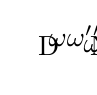
\begin{tikzpicture}
			\tikzset{sibling distance=5pt}
				\Tree	[.DP	\node (3){D};
							[.$\omega$P	\hardNum/\\\hardAdj{}
								[.$\omega'$	\node (2){$\omega$};
								[.NP	Poss
									[.N$'$	\node (1){N};	$\cdots$
									]
								]
								]
							]
						]
				\draw[semithick,->] (1.south west) to [bend left=45] (2.south);
				\draw[semithick,dashed,->] (2.south west) to [bend left=60] (3.south);
			\end{tikzpicture}
		\ex \begin{xlist}
				
					\ex	\gll	tvær stórar bækur Astridar \label{hardarsonND}\\
								two large books Astrid.\hardGen{}\\
						\glt	`two large books of Astrid's'
					\ex	\gll	Hinar tvær stóru bækur (hans) Ottós\label{hardarsonFD}\\
								\hardArt{} two large books \hardProp{} Ottó.\hardGen{}\\
						\glt	`the two large books of Ottó's'
					\ex	\gll	stóru bækur-nar tvær hans Ottós \label{hardarsonBD}\\
								large books-\hardArt{} two \hardProp{} Ottó.\hardGen\\
						\glt	`Ottó's two large books'
			\end{xlist}
\end{multicols}
\end{exe}

In order to determine the possible mechanism behind the fronting of possessors we must first established what is driving movement within the DP. 
I assume that Merge is a last resort operation, which occurs when the derivation would otherwise crash due to unvalued features (cf. \citealt{abels2003,boskovic2007,AgreementLooking:2012wf,Wurmbrand:2013tf,Wurmbrand:2012ty,Wurmbrand:uv,Wurmbrand:2014vz,Wurmbrand:2011ua,Wurmbrand:2013tb}). Hence, the movement of the noun to D and, when applicable, the subsequent movement of the adjective is driven by feature valuation.

Following \cite{Hardarson:2016wd}, N to D movement in Icelandic is the result of an unvalued [R] feature on D, (\ref{hardarsonPatIIIbase}). During the derivation, this feature must then receive its value from a corresponding valued [R] feature elsewhere within the appropriate domain \citep[e.g.,][]{pesetsky2007}. Assuming \textit{Reverse Agree} (Wurmbrand op cit.), the head carrying the valued counterpart of [R] must c-command D. Here, a valued equivalent is carried by $\omega$ \cite[147ff]{Hardarson:2016wd}.\footnote{See \cite[147ff]{Hardarson:2016wd} for a discussion on the nature of this feature.}

Following, e.g. \cite{Matushanski:2006ud} and \cite{Harizanov:2018ep}, I assume that head movement in the syntax operates on par with phrasal movement and that complex heads are formed post-syntactically.\footnote{This could also potentially be carried out via traditional head movement \citep[cf.][]{Hardarson:2016wd}.} In syntax, $\omega$ hence moves to Spec-DP.\footnote{Note that although I present this operation as movement this is done simply for the sake of presentation. Nothing here hinges on whether this operation is movement, copying or remerger.} From this position, $\omega$ c-commands D and values its [\textsc{r}] feature, (\ref{hardarsonNtoD}).

\begin{exe}
\setlength{\columnsep}{-10pt}
\begin{multicols}{2}
	\ex	~ \label{hardarsonPatIIIbase}\\
		\begin{tikzpicture}
			\Tree	[.DP	D\\{$\left[\begin{array}{c}
								{\textsc{r:}\_}\\
								{\textsc{m}}
								\end{array}\right]$}
						[.$\omega$P	{\hardNum}
							[.$\omega'$	{\hardAdj}
								[.$\omega'$	$\omega$\\{[\textsc{r:}$\alpha$]} {$\cdots$}
								]
							]
						]
					]
		\end{tikzpicture}
		\columnbreak
		
	\ex	~ \label{hardarsonNtoD}\\
		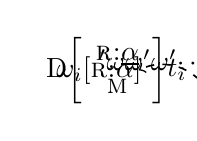
\begin{tikzpicture}
			\Tree	[.DP	\node(1){$\omega_i$\\{[\textsc{r:}$\alpha$]}};
					[.D$'$	\node(2){D\\{$\left[\begin{array}{c}\textsc{r:}\underline{\alpha}\\{\textsc{m}}\end{array}\right]$}};
						[.$\omega$P	{\hardNum}
							[.$\omega'$	{\hardAdj}
								[.$\omega'$	\node(3){$t_i$}; {$\cdots$}
								]
							]
						]
					]
					]
					\draw[semithick,->] (3.south) to [bend left=70] (1.south);
					\draw[semithick,dashed,->] (1.south) to [bend right=45] (2.west);
		\end{tikzpicture}
\end{multicols}
\end{exe}\vspace{-15pt}

\noindent A possible explanation for the choice of head movement in this case, is that phrasal movement is blocked by \textit{Antilocality} \citep[e.g.,][]{Grohmann:2000td,abels2003}.

Post-syntactically D and $\omega$ come to form a complex head through e.g., M-merger \citep{Marantz:1988ug,Matushanski:2006ud}, conflation \citep{Harley:2004ue} or amalgamation \citep{Harizanov:2018ep}. I assume this is triggered by the presence of a feature M present on D \citep[cf.][]{Harley:2004ue,Harizanov:2018ep}. This results in the pattern shown in (\ref{hardarsonPatIII}).

\begin{exe}
	\ex[]{\glll	{\hardN} - {\hardArt} > {\hardNum} > {\hardAdj} \label{hardarsonPatIII}\\
						bækur - nar ~ tvær ~ stóru\\
						books - {\hardArt} ~ two ~ large\\
				\glt	`the two large books'}
\end{exe}

In instances where the adjective also moves to a prearticular position, (\ref{hardarsonBD}), Harðarson \citeyearpar[147ff]{Hardarson:2016wd} argues that the adjective is undergoing focus movement, formalized here as D carrying an unvalued [\textsc{di}(scourse)] feature which is valued by a focus-bearing adjective. In case of fronted possessors, the possessor values both [R] and the [\textsc{di}] features, (\ref{hardarsonfrontposs}). D is then merged into a complex head with the fronted possessor, thus conditioning the null form of the definite D, whose presence is indicated by the weak inflection of the adjectives, see (\ref{hardarsonFrGen}).

\begin{comment}
\begin{exe}
\setlength{\columnsep}{-50pt}
\begin{multicols}{2}
	\ex	~ \label{hardarsonPatIbase}\\
		\begin{tikzpicture}
			\Tree	[.DP	D\\{$\left[\begin{array}{c}
								{\textsc{r:}\_}\\
								{\textsc{di:}\_}\\
								{\textsc{m}}
								\end{array}\right]$}
						[.$\omega$P	{\hardNum}
							[.$\omega'$	{\hardAdj}\\{[\textsc{di:}\textsc{foc}]}
								[.$\omega'$	$\omega$\\{[\textsc{r:}$\alpha$]} {$\cdots$}
								]
							]
						]
					]
		\end{tikzpicture}
		\columnbreak
		
	\ex	~ \label{hardarsonAdjFr}\\
		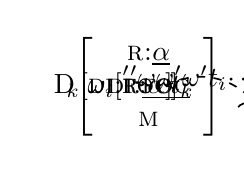
\begin{tikzpicture}
			\Tree	[.DP	\node(4){{\hardAdj$_k$}\\{[\textsc{di:foc}]}};
					[.D$'$	\node(1){$\omega_i$\\{[\textsc{r:}$\alpha$]}};
					[.D$'$	\node(2){D\\{$\left[\begin{array}{c}\textsc{r:}\underline{\alpha}\\{\textsc{di:}\underline{\textsc{foc}}}\\{\textsc{m}}\end{array}\right]$}};
						[.$\omega$P	{\hardNum}
							[.$\omega'$	\node(3){$t_k$};
								[.$\omega'$	$t_i$ {$\cdots$}
								]
							]
						]
					]
					]
					]
					\draw[semithick,->] (3.south west) to [bend left=60] (4.south);
					%\draw[semithick,dashed,->] (1.south) to [bend right=45] (2.west);
					\draw[semithick,dashed,->] (4.south) to [bend right=45] (2.west);
		\end{tikzpicture}
\end{multicols}
\end{exe}
\end{comment}

 

\begin{exe}
%	\ex	~\\
%		\begin{tikzpicture}
		%\tikzset{sibling distance=20pt}
%			\Tree	[.DP	D\\{$\left[\begin{array}{c}
%								{\textsc{r:}\_}\\
%								{\textsc{di:}\_}\\
%								{\textsc{m}}
%								\end{array}\right]$}
%						[.$\omega$P	{\hardNum}
%							[.$\omega'$	{\hardAdj}
%								[.$\omega'$	$\omega$
%											[.NP	D$_\hardGen$\\{$\left[\begin{array}{c}
%																{\textsc{r:$\beta$}}\\
%																{\textsc{di:foc}}
%																\end{array}\right]$} $\cdots$
%											]
%								]
%							]
%						]
%					]
%		\end{tikzpicture}

	\ex ~ \label{hardarsonfrontposs}\\
		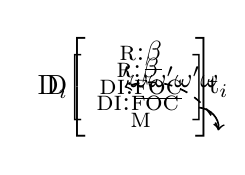
\begin{tikzpicture}
			\tikzset{sibling distance=20pt}
			\Tree	[.DP	\node(2){D$_{\hardGen i}$\\{$\left[\begin{array}{c}
										{\textsc{r:$\beta$}}\\
										{\textsc{di:foc}}
										\end{array}\right]$}};
											[.D$'$	\node(3){D\\{$\left[\begin{array}{c}
														{\textsc{r:\underline{$\beta$}}}\\
														{\textsc{di:\underline{foc}}}\\
														{\textsc{m}}
														\end{array}\right]$}};
													[.$\omega$P	{\hardNum}
																[.$\omega'$	{\hardAdj}
																	[.$\omega'$	$\omega$
																		[.NP	\node(1){t$_i$}; N
																		]
																	]
																]
													]
											]
					]
						\draw[semithick,->] (1.south west) to [bend left=45] (2.south);
						%\draw[semithick,dashed,->] (1.south) to [bend right=45] (2.west);
						\draw[semithick,dashed,->] (2.south) to [bend right=45] (3.west);
		\end{tikzpicture}
\end{exe}

\noindent This approach does capture the fact that fronting these possessors does require contrastive focus and blocks the movement of the noun and adjectives, (\ref{hardarsonFrGen}).\footnote{Under this, Spec-DP of a definite DP would be a criterial position \citep[cf.][]{Rizzi:2006ti,Boskovic:2008wp,wurmbrand2014gisli,wurmbrand2015}. The unavailability of subextraction of adjectives and genitives would follow, as movement to spec-DP would freeze them for the purposes of any subsequent criterial movement, such as topicalization, focus movement, or quantifier raising. See section 3 for some further evidence for this position.}

\begin{exe}
\ex	\label{hardarsonFrGen}
	\begin{xlist}
	\ex[]{	\gll	Astrid-ar (*(h)inar) tvær stóru bækur\\
					Astrid-{\hardGen} \hardArt{} two large. books\\
			\glt	`Astrid's two large books'		
		}
	\setlength{\columnsep}{20pt}
	\begin{multicols}{2}
	\ex[*]{	\gll	Astrid-ar bækur tvær stóru\\
					Astrid-{\hardGen} books two large\\
			\glt
		}%\columnbreak
	\ex[*]{	\gll	Astrid-ar stóru bækur tvær\\
					Astrid-{\hardGen} large books two\\
			\glt
		}%\vspace{-1.1\baselineskip}
	\end{multicols}
	\end{xlist}
\end{exe}

There are two issues, however, that are not adequately addressed in \cite{Hardarson:2016wd}: one being the branchingness effects, and the other being the minimality violation in fronting the possessor rather than the noun and adjective.

Turning first to the branchingness effects, there are two main questions: how is it possible perform head movement from a specifier position, and why is it not possible to strand modifiers as in typical cases of head movement?

To address these questions, let us first examine the formation of the noun. The full structure of the Icelandic DP under \cite{Hardarson:2016wd} is shown in (\ref{hardarsonFull}). As mentioned above, the noun is argued to be formed through the accumulation of the heads up to $\omega$ (\ref{hardarsonFull}) and in certain definite DPs, including D, which results in the complex head shown in (\ref{hardarsonFullN}).

\begin{exe}
%\setlength{\columnsep}{-5pt}
\begin{multicols}{2}
		\ex	~ \label{hardarsonFull}\\
			\begin{tikzpicture}
			\tikzset{sibling distance=20pt}
				\Tree	[.DP	D
							[.$\omega$P	$\omega$
								[.$\varphi$P	$\varphi$
									[.nP	n	$\sqrt{\textsc{root}}$
									]
								]
							]
						]
			\end{tikzpicture}
		\ex	~ \label{hardarsonFullN} \\
			\begin{tikzpicture}
			\tikzset{sibling distance=15pt}
			\tikzset{level distance=20pt}
			\Tree	[
					[
						[
							[	$\sqrt{\textsc{root}}$	n
							] $\varphi$
						] $\omega$
					] D
				]
			\end{tikzpicture}
	\end{multicols}

\end{exe}

\noindent The configuration shown in (\ref{hardarsonFull}--\ref{hardarsonFullN}) introduces a redundancy. Under traditional assumptions regarding the formulation of complex heads and merge, the heads necessarily form a phrasal construction prior to the formulation of the complex head. In the absence of any DP-internal modifiers, these operations apply vacuously. This redundancy has been used as an argument for \textit{Spanning}, i.e. vocabulary insertion targeting non-terminal nodes \citep[e.g.,][]{svenonius2016}.

However, under \textit{Bare Phrase Structure Grammar} \citep{Chomsky:1995uq}, is possible to merge two heads and form a complex head directly. This possibility has been utilized, e.g., for the formation of compounds \citep[e.g.,][]{Josefsson:1997te,josefsson1998,zhang2007,Siddiqi:2009tm,okubo2013,Hardarson:2018vo}. \cite{hardarson2020} also makes use of this possibility in addressing patterns in the distribution of Penultimate Vowel Lengthening in Zulu discussed by Cheng and Downing (\citeyear{Cheng:2007um} et seq.). There it is argued that when two unmodified heads are merged, i.e., neither of them has projected to a phrase, with one or both of them carrying an M feature, a complex head is formed directly without first forming a phrase. If either of the heads is modified, i.e. has projected to a phrase, the merger will result in a phrasal construction and the formation of the complex head will take place post-syntactically. This is schematized below.\footnote{Note that both heads are M-marked below in order to abstract away from the directionality of the process. That may not be necessarily.}

\begin{exe}
	\ex	 	{Merger of two unmodified \textsc{m}-marked heads} \citep[468]{hardarson2020} \label{hardarsonhead}
			\begin{xlist}
	  		\sn	{Y$_{\textsc{m}}$ + X$_{\textsc{m}}$ $\rightarrow$ [$_{\mathrm{X}}$ Y X]}
			\end{xlist}
	\ex	Merger of two \textsc{m}-marked heads with modification \citep[468]{hardarson2020} \label{hardarsonhead+}
		\begin{xlist}
			\ex	Raising\\
				Y$_{\textsc{m}}$ + [$_{\mathrm{XP}}$ X$_{\textsc{m}}$ ZP] $\rightarrow$ [$_{\mathrm{YP}}$ Y$_{\textsc{m}}$ [$_{\mathrm{XP}}$ X$_{\textsc{m}}$ ZP]] $\rightarrow$ [$_{\mathrm{YP}}$ [$_{\mathrm{Y}}$ Y+X] [$_{\mathrm{XP}}$  ZP]]
			\ex Lowering\\
				Y$_{\textsc{m}}$ + [$_{\mathrm{XP}}$ X$_{\textsc{m}}$ ZP] $\rightarrow$ [$_{\mathrm{YP}}$ Y$_{\textsc{m}}$ [$_{\mathrm{XP}}$ X$_{\textsc{m}}$ ZP]] $\rightarrow$ [$_{\mathrm{YP}}$  [$_{\mathrm{XP}}$ [$_{\mathrm{X}}$ Y+X]  ZP]]
		\end{xlist}
\end{exe} 


\noindent The argument carries over to the Icelandic DP. As discussed above, the heads in the extended nominal projection come to form a complex head. Hence, in the absence of modifiers, the complex head in (\ref{hardarsonFullN}) can be formed directly under (\ref{hardarsonhead}), without first forming the phrasal configuration in (\ref{hardarsonFull}). Performing head movement out of the specifier is then no longer an issue. This is not a head movement out of a specifier, but a head movement of an entire specifier. The possessor can then satisfy all the requirements of the matrix D, including serving as its host, and subsequently conditioning the null form of D. This allows us to exclude stranding of modifiers given the difficulty of subextraction from specifiers in general.

A possible way of ruling out phrasal movement of the possessor may lie in an inversion of the last resort condition of movement, i.e., that Merge does not occur if it leads to features not being satified. As mentioned above, the fronted possessor values both the [R] and the [\textsc{di}] features, preventing the movement of both the head noun and the adjectives. Note, however, although this would mean introducing some form of optimization into the derivation, the optimization in this case is local in that it only evaluates possibilities for the next step in the derivation \citep[cf.][]{heck2007,Lahne:2009va}. In the case of the modifier-less possessors, they are also able to satisfy D's [M] feature by virtue of being a nominal head c-commanding D. If a phrasal element were to move to this position, it would be able to value both [R] and the [\textsc{di}] features and prevent movement of nouns and adjectives, just as the modifier-less. However it would not provide a suitable host for the matrix D as there is no head c-commanding it, thus not satisfying the [M] feature.

Turning to the minimality effects, one possibility is that Agree prioritizes single agree over multiple agree, and when an element that can value all of the relevant features us accessible, that element will be targeted over closer elements that only partially satisfy the unvalued features of the head. This would mean that, as the focused unmodified possessors can satisfy all three of the relevant features, it will be given priority over the head noun and the adjective, which only partially satisfy the features of D.

To summarize this section, the branchingness effects that are observed with definite possessors can be accounted for under the proposal in \cite{hardarson2020}: In the absence of any modifiers, a definite DP will form a single head, hence allowing it to value all the features of the matrix D and serve as a host for D. In the presence of modifiers, the possessor forms a phrase, and can still value the relevant features of D, but cannot serve as a host.


\section{Quantified possessors}

Turning to the quantified possessors, as mentioned above, these differ from the definite possessors in a number of ways: first, they contain modifiers, as discussed above, and thus would be considered phrasal under the approach taken here. Second, their fronting is not limited to occurring within definite DPs, but they can also be fronted within indefinite DPs. Third, the fronted definite possessors carry focus and obligatory contrastive stress, the quantified possessors do not. And fourth, the position of the possessor relative to other material in the DP has semantic consequences beyond what is observed with the definite possessors.

Just as we saw with the definite possessors, there appear to be two possible positions for quantified possessors within the DP, postnominal and prenominal, (\ref{hardarsoninnie-QR}--\ref{hardarsoninnieDef}). In addition to that, the position is relevant for the availability of different scope readings.

For the indefinite DPs, when the possessor follows the noun, (\ref{hardarsonindef-postnom}), the DP is ambiguous with respect to the two possible readings: either there is i) a particular large bunny that belongs to each of the children ($\exists \gg \forall$), or ii) each child has their respective large bunny ($\forall \gg \exists$). When the possessor is fronted, (\ref{hardarsonindef-preadj}), this ambiguity is lost and the only reading possible is reading (ii).\footnote{
Note that it is possible for a quantified possessor to occur between the adjective and noun, (\ref{hardarsonindef-postadj}--\ref{hardarsondef-postadj}). This position also freezes the scope possibilities for the QP, as shown.

\begin{exe}
\settowidth\jamwidth {*\textsc{Det} $\gg \forall$; $\forall \gg$ \textsc{Det}}
	\ex	\gll	stór-$\emptyset$ [hver-s barn-s] kanína \label{hardarsonindef-postadj}\\
					large-{\hardStr} ~each-{\hardGen} child-{\hardGen} bunny\\ \jambox{$\exists \gg \forall$; *$\forall \gg \exists$}
			\glt
		\ex	\gll	hin stór-a [hver-s barn-s] kanína \label{hardarsondef-postadj}\\
						{\hardArt} large-{\hardWk} ~each-{\hardGen} child-{\hardGen} bunny\\ \jambox{\textsc{Det} $\gg \forall$; *$\forall \gg$ \textsc{Det}}
				\glt
\end{exe}

There is, however, reason to believe this may not be a phrasal construction. First there is an absence of a prosodic break between the genitive and the head noun, which occurs with other genitives, and second, the stress pattern is more akin to compound stress, with primary stress on the quantifier and secondary stress on the first syllable of the head noun. Hence it is possible that this may be a case of phrasal compound, which may also explain the semantic effects. If it is a part of a complex head, it cannot move to spec-DP on its own.}
This indicates that from its position in (\ref{hardarsonindef-preadj}), the possessor c-commands whatever is carrying the existential force of the DP.

\begin{exe}
\settowidth\jamwidth {*$\exists \gg \forall$; $\forall \gg \exists$}
\ex	\label{hardarsoninnie-QR}
	\begin{xlist}
		\ex	\gll	stór-$\emptyset$ kanína [hver-s barn-s] \label{hardarsonindef-postnom}\\
					large-{\hardStr} bunny	~each-{\hardGen} child-{\hardGen}\\ \jambox{$\exists \gg \forall$; $\forall \gg \exists$}
			\glt	`each child's large bunny'  
	
		\ex	\gll	{[}hver-s barn-s] stór-$\emptyset$ kanína \label{hardarsonindef-preadj}\\
					~each-{\hardGen} child-{\hardGen} large-{\hardStr} bunny\\ \jambox{*$\exists \gg \forall$; $\forall \gg \exists$}
			\glt 	
	\end{xlist}
\end{exe}

\noindent Assuming that the existential force of indefinite DPs is a property of determiners  \citep[cf.][]{chierchia1992}, the available scope indicates that the possessor is situated in Spec-DP in (\ref{hardarsonindef-preadj}). The differences in meaning then result from the possessor taking wide or narrow scope with respect to D.\footnote{Furthermore, in the light of (\ref{hardarsoninnie-QR}) and (\ref{hardarsoninnieDef}), this indicates that there is in fact a null D in indefinite DPs in Icelandic, contra \cite{Hardarson:2016wd}.} The ambiguity of the DPs in which the possessor remains in situ in turn indicates that this movement also occurs covertly.

\begin{exe}
    %\setlength{\columnsep}{-55pt}
    \begin{multicols}{2}
    \ex $\exists \gg \forall$; $\forall \gg \exists$\\
        \begin{tikzpicture}
            \Tree   [.DP    D$_{\exists}$
                            [.$\omega$P \textsc{large}
                                [.$\omega'$  $\omega$\\\textsc{bunny}
                                    [.NP    \textsc{$\forall$ child} $\cdots$
                                    ]
                                ]
                            ]
                    ]
        \end{tikzpicture} \columnbreak
    \ex *$\exists \gg \forall$; $\forall \gg \exists$\\
        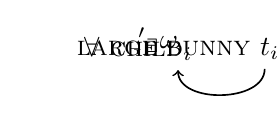
\begin{tikzpicture}
            \Tree   [.DP    \node (1){\textsc{$\forall$ child}$_i$};
                            [.D$'$ D$_{\exists}$
                            [.$\omega$P \edge[roof]; \node (2) {\textsc{large} \textsc{bunny} $t_i$};
                            ]
                            ]
                    ]
                    %\node (DP1) [below=1pt of 1] {};
                    %\node (DP2) [below,xshift=1cm of 2] {};
                    \draw[semithick,->] ([xshift=1.1cm]2.south) [out=-90,in=-90,looseness=1] to (1.south);
        \end{tikzpicture}
    \end{multicols}
\end{exe}

For definite DPs, the same pattern is observed. When the possessor is postnominal, (\ref{hardarsondef-postnom}), the DP is ambiguous: i) there is a single large bunny that belongs to each child (\textsc{Det} $\gg \forall$), or ii) each child respectively has a single bunny that is large ($\forall \gg$ \textsc{Det}). If the possessor is fronted, (\ref{hardarsondef-preadj}), this ambiguity is lost, and only reading (ii) is available.\footnote{Note that although the definite article has a null form in (\ref{hardarsondef-preadj}), the DP can be identified as definite by the weak adjective inflection, which occurs within (formally) definite DPs. Precisely what is conditioning the null form, however, is not entirely clear.}

\begin{exe}
     \settowidth\jamwidth {*\textsc{Det} $\gg \forall$; $\forall \gg$ \textsc{Det}}
	\ex	\label{hardarsoninnieDef}
		\begin{xlist}
			\ex[]{\gll	hin stór-a kanína [hver-s barn-s] \label{hardarsondef-postnom}\\
						{\hardArt} large-{\hardWk} bunny ~each-{\hardGen} child-{\hardGen}\\ \jambox{\textsc{Det} $\gg \forall$; $\forall \gg$ \textsc{Det}}
				\glt	}

			\ex	\gll	{[}hver-s barn-s] stór-a kanína \label{hardarsondef-preadj}\\
						~each-{\hardGen} child-{\hardGen} large-{\hardWk} bunny\\ \jambox{*\textsc{Det} $\gg \forall$; $\forall \gg$ \textsc{Det}}
				\glt
		\end{xlist}
\end{exe}

Hence, it would appear that the possessor is moving to Spec-DP by way of overt quantifier raising.

Another relevant point of difference between the quantified genitives and other genitives is that they appear to be extractable out of the DP, albeit not overtly. Overt subextraction from DPs is generally limited to argument PPs, (\ref{hardarsonargPP}) or their complements, (\ref{hardarsonagrcompl}). Overt extraction out of definite DPs is generally ruled out, (\ref{hardarsondefno}).\pagebreak

\begin{exe}
	\ex	\citep[197]{Hardarson:2016wd}
		\begin{xlist}
			\ex[?]{	\gll	[Á hverjum]$_i$ vannstu [sigur $t_i$]?\label{hardarsonargPP}\\
							~on who won.you victory\\
					\glt	`Who did you defeat?'
					}
			\ex[]{	\gll	Hverjum$_i$ vannstu [sigur [á $t_i$]]?\label{hardarsonagrcompl}\\
							who won.you victory on\\
					\glt	}
			\ex[*]{	\gll	Hverjum vannstu [sigurinn [á $t_i$]]?\label{hardarsondefno}\\
							who won.you victory.{\hardArt} on\\ }
		\end{xlist}
\end{exe}

\noindent Overt extraction of possessors is not possible in Icelandic, (\ref{hardarsonOvert-movt}). However, the availability of different scope readings indicate that it is possible for covert extraction to take place (\citealt{Hardarson:2016wd}). This is shown in (\ref{hardarsonQR}) below where the possessor to takes wide scope over the subject (see also \citealt{Wurmbrand:2008wc,Bobaljik:va} for a similar effect in German).

\begin{exe}
	\ex[]{\citep[200]{Hardarson:2016wd} \label{hardarsonOvert-movt}} \vspace{-5pt}
	\sn[*]{\gll	Hvers$_i$ horfðir þú á [sigur $t_i$ á Svíum]\\
				who.{\hardGen} wathced you on ~victory ~ on Swedes\\
		\glt	Int:`Whose victory over the Swedes did you watch?' }
	\ex[]{\citep[201, ad.]{Hardarson:2016wd} \label{hardarsonQR}\\
		\gll	{[}Einn stúdent] borðaði [kanínu [hver-s barn-s]]\\
				~one student ate bunny each-{\hardGen} child-{\hardGen}\\
		\glt
			\begin{xlist}
				\ex[]{`A single student ate all the children's bunnies.' \hfill $\exists \gg \forall$
}
				\ex[]{`Each child is such that a student ate their bunny.' \hfill $\forall \gg \exists$}
			\end{xlist}}
\end{exe}

\noindent It is worth noting at this point that under \cite[22ff]{Kayne:1994uo} specifiers are argued to c-command out of their phrases, hence this does beg the question of whether this is really a case of covert extraction of the possessor or if this is rather a matter of covert movement to Spec-DP and subsequent pied piping. We saw in (\ref{hardarsonindef-postnom}) and (\ref{hardarsondef-postnom}), that if scope readings are the result of different c-command relationships, covert movement to Spec-DP does take place. If it were the case that the wide scope of the possessor in (\ref{hardarsonQR}) is the result of movement to Spec-DP and subsequent pied piping, we would expect all prenominal possessors to be able to license material outside of the DP via c-command. Binding facts show that this is not the case, i.e., possessors in Spec-DP do not c-command out of the DP.

Non-quantified possessors, whether pre- or postnominal, do not licence a reflexive pronoun, (\ref{hardarsonunbound}). This strongly indicates that a possessor does not c-command out of the DP whether it is overtly or potentially covertly positioned in spec-DP. Note, however, that the DP containing the possessor can serve as an antecedent for the reflexive pronoun. The structure for (\ref{hardarson*self}) is provided in (\ref{hardarson*selfstr}) below, where the TP, vP, and VP layers have been omitted.

\begin{exe}
	\ex	\label{hardarsonunbound} 
		\begin{xlist}
			\ex[]{	\gll	{[}Kanína Astridar$_i]_j$ leitar að [pabba sínum$_{*i/j}$]\\
							~bunny Astrid.{\hardGen} seeks at ~dad self's\\
					\glt	`Astrid's bunny is looking for her dad.'}
			\ex[]{	\gll	{[}Astridar$_i$ kanína]$_j$ leitar að [pabba sínum$_{*i/j}$]\\
							Astrid.{\hardGen} bunny seeks at ~dad self's\\
					\glt	}\label{hardarson*self}
		\end{xlist}
\end{exe}\vspace{-10pt}

\begin{exe}
	\ex	The structure of (\ref{hardarson*self})\label{hardarson*selfstr}\\
		\begin{tikzpicture}
			\Tree	[.CP	[.DP$_j$	\textsc{astrid}$_i$
								[.D$'$	D
								[.$\omega$P $\omega$\\\textsc{bunny} $\cdots$
								]
								]
							]		[.C$'$	C\\\textsc{seek}
												[.$\cdots$	
																	[.PP	P\\\textsc{at}
																		[.DP	D
																			[.$\omega$P $\omega$\\\textsc{dad}
																				[.NP	\textsc{self}$_{*i/j}$
																					 $\cdots$
																				] 
																			]
																		]
																	]
												]
									]
					]
		\end{tikzpicture}
\end{exe}

\noindent This effect cannot be explained as a matter of domains, i.e., it cannot be the case that the possessor is unable to license the reflexive due to the reflexive being embedded within an inaccessible domain in the structure in (\ref{hardarson*selfstr}). If that were the case, we would expect that the DP containing the possessor would also fail to license the reflexive as it is no less distant from the DP containing the possessor in terms of domains. This is not the case and hence this indicates that possessors do not c-command from their position in Spec-DP.

Turning back to the quantified possessors, when they are in a postnominal position they can bind a pronoun and give rise to a bound variable reading. This is shown in (\ref{hardarsonBV}), where the possessor is able to bind a variable that is overtly c-commanded by its matrix DP. The structure of (\ref{hardarsonBV}) is given in (\ref{hardarsonObvstr}) below.

\begin{exe}
	\ex	\gll {[}foreldri [hvers barns]$_i$] er með [mynd [af því$_{i/k}$]] uppi í hillu. \label{hardarsonBV}\\
			~parent ~each.{\hardGen} child.{\hardGen} is with ~picture ~of it up in shelf\\
		\glt	`Each child's parent has their picture up on their shelf.' \hfill \textsc{bv}
\end{exe}

 

\begin{exe}
    \ex The overt structure of (\ref{hardarsonBV}) \label{hardarsonObvstr}\\
        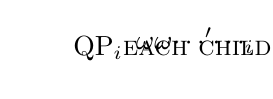
\begin{tikzpicture}
		\Tree	[.CP	[.DP D
								[.$\omega$P $\omega$\\\textsc{parent}
									[.NP	\node (1){QP$_i$\\{\textsc{each child}}}; $\cdots$
									]
								]
							]
							[.C$'$	C	[.TP \edge[roof]; {$\cdots$ \textsc{picture of \textbf{it}}$_i$} ]
							]
				]
	    \end{tikzpicture}
\end{exe}

\noindent Assuming that the bound variable reading requires a c-commanding antecedent (\citealt{Reinhart:1983vx}), the bound variable reading should be impossible under the structure in (\ref{hardarsonObvstr}), as possessors do not license reflexives from their position within the DP. Hence the fact that the bound variable reading is possible indicates that the possessor must move out of the DP to a position c-commanding the variable, (\ref{hardarsonbvstr}).

\begin{exe}
	\ex	Structure of (\ref{hardarsonBV}) at LF \label{hardarsonbvstr}\\
	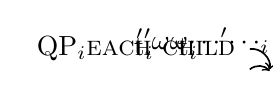
\begin{tikzpicture}
		\Tree	[.CP	\node (3){QP$_i$\\{\textsc{each child}}};
					[.C$'$	[.DP \node (2){t$_i$};
							[.D$'$ D
								[.$\omega$P $\omega$\\\textsc{parent}
									[.NP	\node (1){t$_i$}; $\cdots$
									]
								]
							]
							]
							[.C$'$	C	[.TP \edge[roof]; {$\cdots$ \textsc{picture of \textbf{it}}$_i$} ]
							]
					]	
				]
				\draw[semithick,->] (1.west) to [bend left=55] (2.south);
				\draw[semithick,->] (2.south west) to [bend left=45] (3.south);
	\end{tikzpicture}
\end{exe}


However, if the possessor has been fronted, i.e., if it has overtly moved to Spec-DP, the bound variable reading is lost, (\ref{hardarson*BV}). This indicates that whatever movement that is responsible for the fronting of the possessor, also freezes the possessor for the purposes of subsequent movement.\footnote{\cite{carminati2002} provide some experimental evidence that challenges the view that bound variable anaphora require a c-commanding antecedent and propose that bound variable reading in the absence of a c-commanding antecedent is an instance of an anaphoric pronoun with an inferred antecedent. However, this study does not rule out potential covert raising of the quantifier in the context of embedding or coordination, which could establish c-command relation between the QP and the variable. Furthermore, this would fail to predict the scope differences that are observed between (\ref{hardarsonBV}--\ref{hardarson*BV}), as there is no clear reason for why an inferred antecedent coreferential with the possessor would be less available when the possessor is prenominal.}

\begin{exe}
	\ex	\gll	{[}[hvers barns]$_i$ foreldri] er með [mynd [af því$_{*i/k}$]] uppi í hillu.\label{hardarson*BV} \\
			~~each.{\hardGen} child.{\hardGen} parent  is with ~picture ~of it up in shelf\\
		\glt	`Each child's parent has their picture up on their shelf.' \hfill \textsc{*bv}
\end{exe}

\noindent Furthermore, if fronting freezes the possessor for further movement, the expectation is that it should be frozen for quantifier raising as well. This prediction is borne out, as shown in (\ref{hardarson*QR}).

\begin{exe}
	\ex	\gll	{[}Einn stúdent] borðaði [[hvers barns] kanínu].\label{hardarson*QR}\\
				~~one student ate ~~each.{\hardGen} child.{\hardGen} bunny\\
		\glt
			\begin{xlist}
				\ex[]{`A single student ate all the children's bunnies.' \hfill $\exists \gg \forall$
}
				\ex[*]{`Each child is such that a student ate their bunny.' \hfill *$\forall \gg \exists$}
			\end{xlist}
\end{exe}

This is consistent with the proposal above, that the fronting of the quantified possessor is an instance of DP-internal quantifier raising. As such, once the movement has occurred, the possessor is frozen for the purposes of further quantifier raising, whether overt or covert. When the possessor is overtly in situ, it is free to raise covertly to either Spec-DP, or beyond the DP. This is consistent with the notion of criterial freezing \citep{Rizzi:2006ti,wurmbrand2014gisli,wurmbrand2015}, i.e., criterial movement, such as quantifier raising, focus movement, a.o., prevents any subsequent criterial movement.

To summarize this section, the fronting of quantified possessors appear to be a case of overt quantifier raising, where the position of the possessor affects the interpretation of the DP. This analysis is further supported by the fact that quantified possessors can be covertly extracted for interpretative purposes as well, whereas fronting of the possessor prevents subextraction. This is consistent with theories in which movement prevents subsequent movement for the same purposes.




\section{Conclusions}

Much ground still remains to be covered when it comes to the internal syntax of the Icelandic DP. Staying close to the topic at hand, one aspect that remains to be explored are the properties of the non-possessor genitives, their positions within the DP and their mobility. This includes the midfield genitives, which appear to have a distribution similar to adjectives, and other argument genitives. Unfortunately, due to restrictions on both time and space, these will have to left for future research.

To summarize the ground covered in this chapter, I have discussed two types of DP-internal possessor fronting. The different criteria for the two types were argued to follow from mechanisms already in place, i.e., feature valuation, word formation, and quantifier raising. The feature valuation approach has been argued for in \cite{Hardarson:2016wd} in order to account for other word order effects within the Icelandic DP. With the amendments proposed here, the fronting of definite possessors can be fully integrated into that analysis and provides an explanation for the size restrictions observed. In the case of the quantified possessors, their fronting appears to be an instance of overt quantifier raising, where the possessor takes scope over the determiner. This was also shown to interact with the availability of covert subextraction of quantified possessors, where if they raise to Spec-DP overtly, they cannot be extracted covertly.




\section*{Abbreviations}
\begin{tabularx}{.45\textwidth}{lQ}
\hardArt & article \\
\hardAdj & adjective \\
\hardNum & numeral   \\
\end{tabularx}
\begin{tabularx}{.45\textwidth}{lQ}
\hardProp & proprial article \\
\hardStr & strong inflection \\
\hardWk & weak inflection\\
\end{tabularx}

\section*{Acknowledgements}
For discussions and comments on various aspect and iterations of this work as well as judgements, I would like to thank Jim Wood, Einar Freyr Sigurðsson, Íris Edda Nowenstein, Jane Middleton, Höskuldur Þráinsson, Þórhallur Eyþórsson, Jóhannes Gísli Jónsson, the audience at the University of Iceland Humanities Congress 2019, and, of course, the anonymous reviewer and the editors of this volume.

\printbibliography[heading=subbibliography,notkeyword=this]

\end{document}